\part{Cloud Foundry Basics}

\begin{frame}{From Traditional Development to PaaS}
\begin{columns}[T] 
\begin{column}{.53\textwidth}
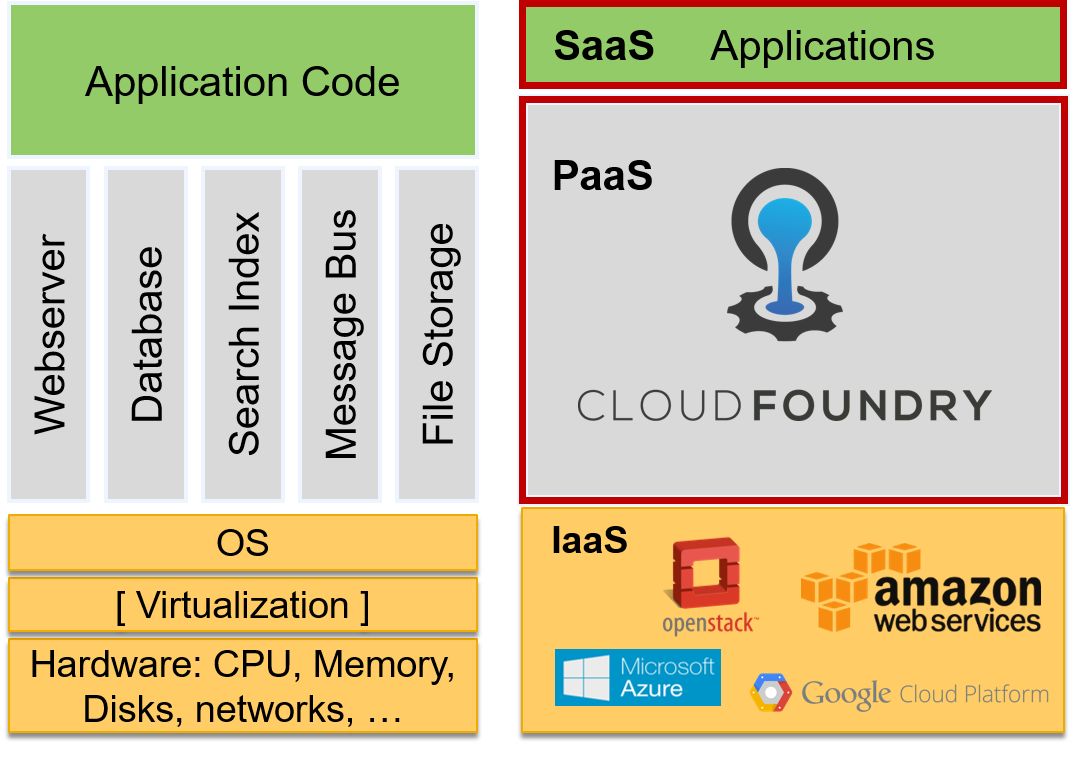
\includegraphics[width=1\textwidth]{../CloudFoundryBasics/images/CF_Basics_1_PaaS_Intro}
\end{column}
\hfill
\begin{column}{.47\textwidth}
\only<2>{\small
    \textbf{SaaS (Software-as-a-Service)} \\focusses on implementing valuable services in problem domain
    \newline
    \textbf{PaaS (Platform-as-a-Service)} \\manages (configures, deploys, scales, upgrades) highly available applications
    \newline
    \textbf{IaaS (Infrastructure-as-a-Service)} \\offers on-demand seemingly infinite resources \& seamless failover
}
\end{column}
\end{columns}
\end{frame}

\begin{frame}{SAP (public) Cloud Platforms}{\colorlink{https://jam4.sapjam.com/groups/about_page/ZBxGNs1cJ5Z7OVkQRwBM0G}{OneCP JAM}}
\includeGraphicsSAPCloudPlatforms{width=1.0\textwidth}
\vfill
\small
\colorlink{https://help.sap.com/viewer/65de2977205c403bbc107264b8eccf4b/Cloud/en-US/350356d1dc314d3199dca15bd2ab9b0e.html}{SAP Cloud Platform - Regions and Hosts}
\end{frame}


\begin{frame}{What is Cloud Foundry?}
	\begin{figure}
  	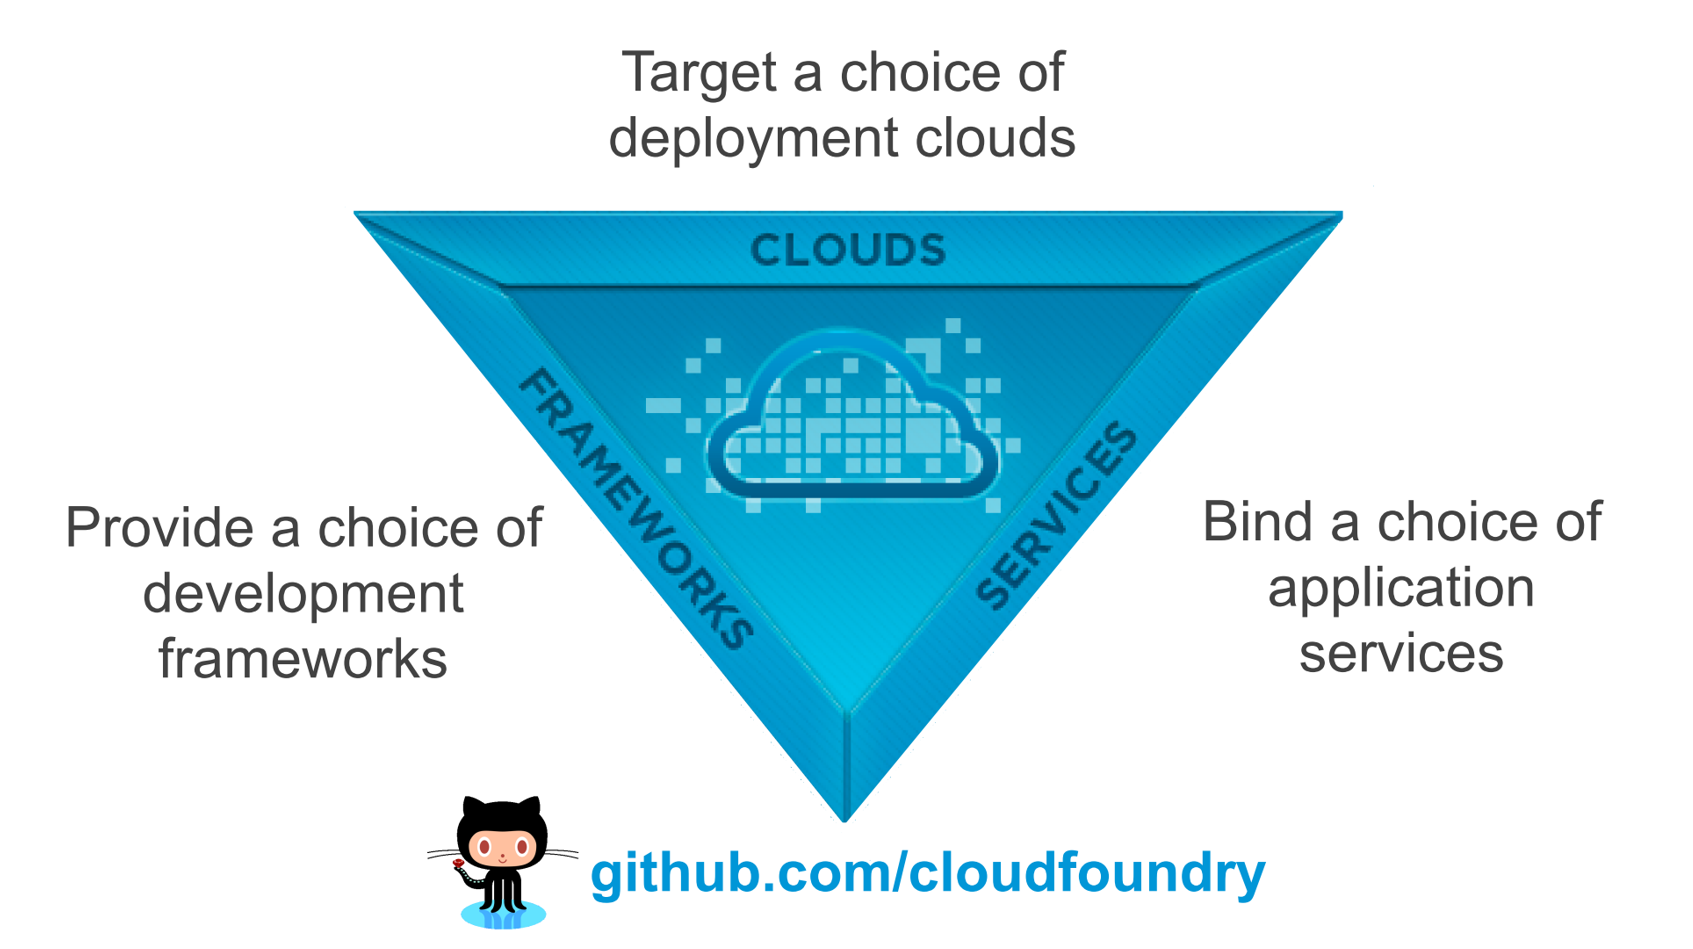
\includegraphics[width=1.0\textwidth]{../CloudFoundryBasics//images/CF_Basics_2_CF_Intro1}
	\end{figure}
\end{frame}


\begin{frame}{Many Languages, Providers and Backing Services}
	\begin{figure}
  	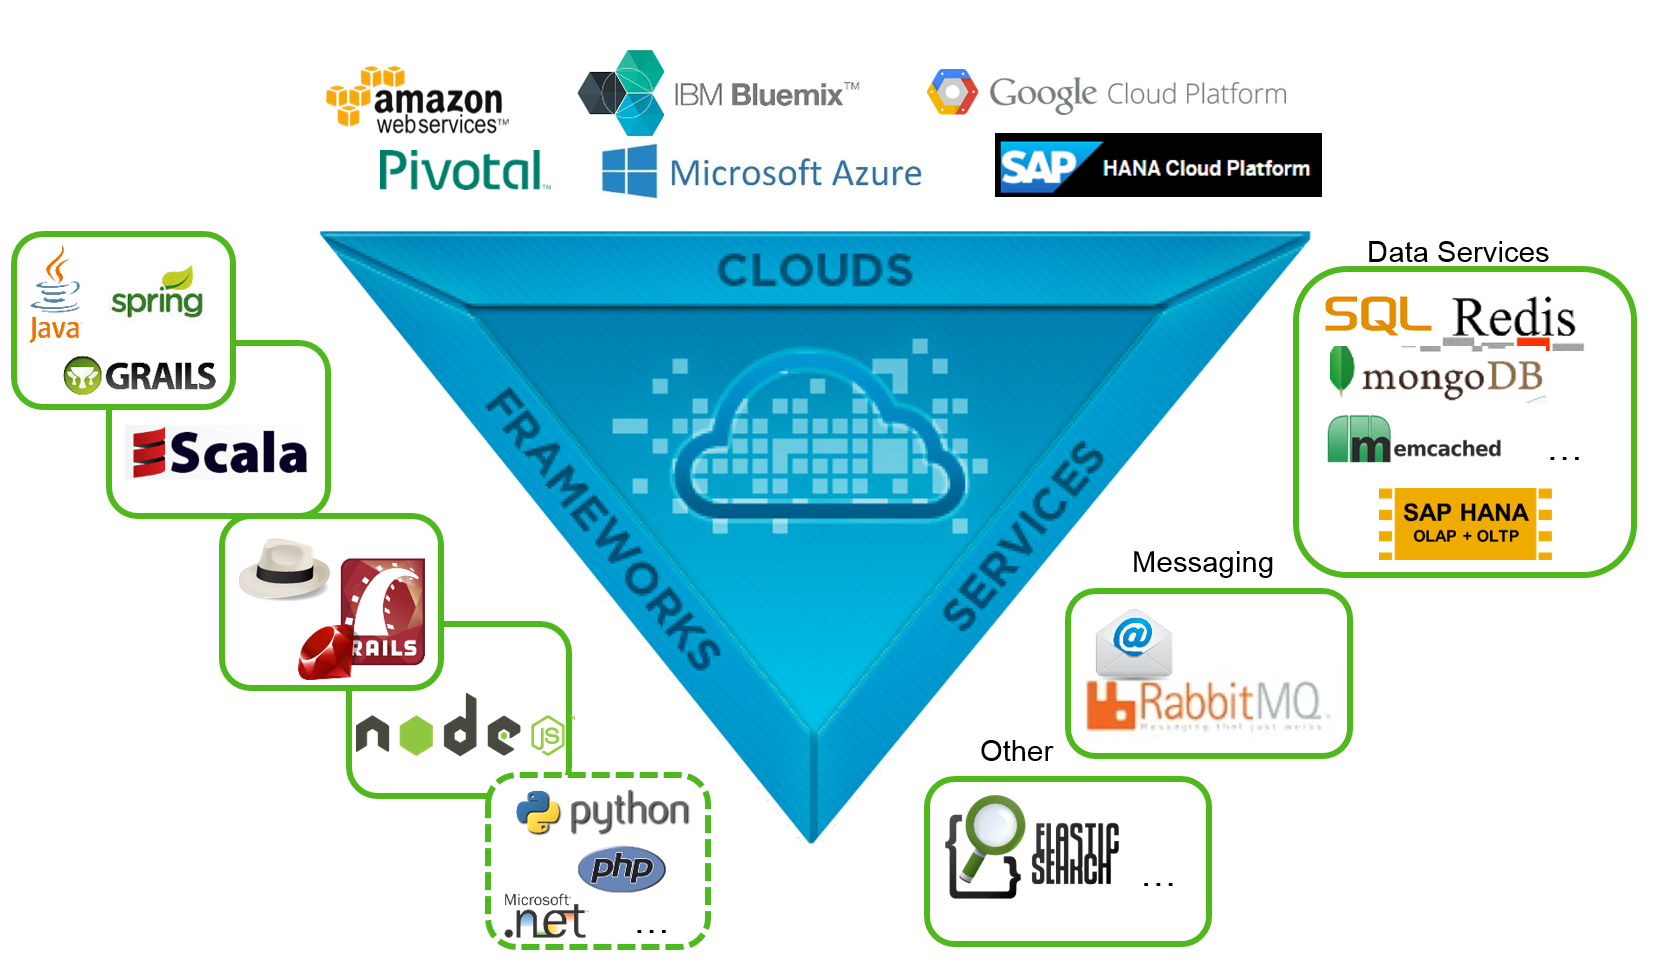
\includegraphics[width=1.0\textwidth]{../CloudFoundryBasics//images/CF_Basics_3_CF_Intro2}
	\end{figure}
\end{frame}


\begin{frame}{SAP's CP Extension to Cloud Foundry}
Cloud Foundry providers differ in the backing services they offer
	\begin{figure}
  	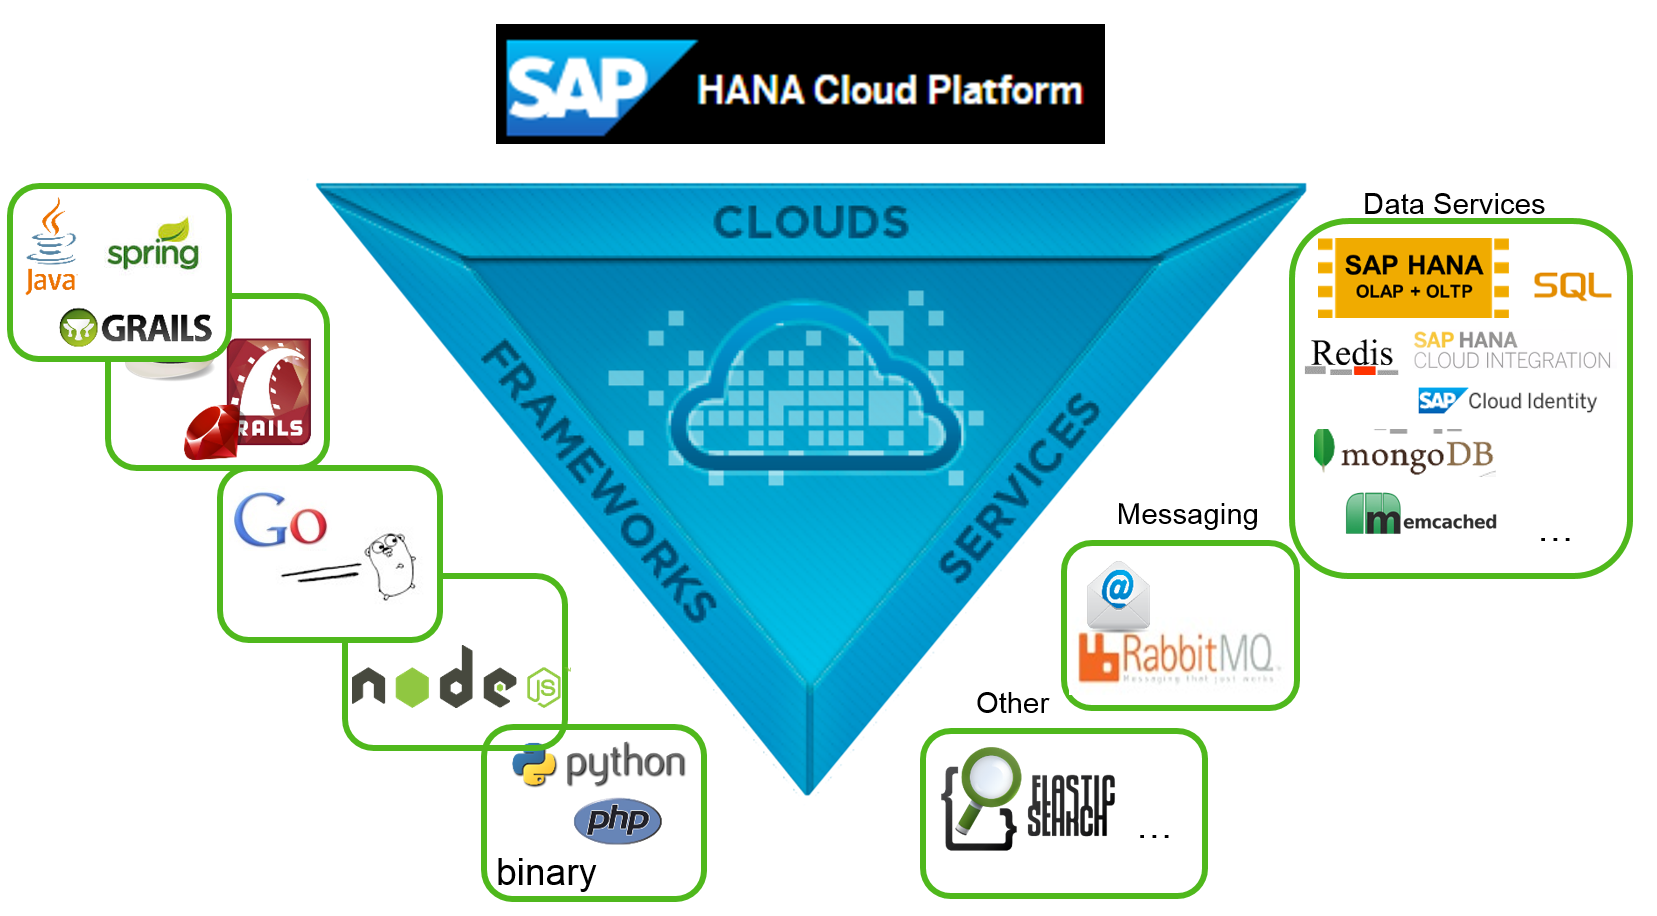
\includegraphics[width=0.9\textwidth]{../CloudFoundryBasics//images/CF_Basics_3b}
	\end{figure}
\end{frame}


\begin{frame}{Key Elements of a PaaS / Cloud Foundry}
	A PaaS (Platform-as-a-Service) is the foundation of your application that supports
	\begin{itemize}[<+->]
		\item \textbf{Multiple languages} (use what fits best): Java, Node, Go, \dots
		\item \textbf{Many backing services}: SQL, No-SQL, Messaging, Blobstore, \dots
		\item \textbf{Resilience}: High availability, no single-point-of-failure, self-healing
		\item \textbf{Virtualized resources}: CPUs, memory, disks, networks, routers, \dots
		\item \textbf{Boundless scalability}: need to program differently
		\item \textbf{Monitoring}: detailed transparency on load and issues
		\item \textbf{Simple deployment}
	\end{itemize}
\end{frame}


\begin{frame}{Cloud Foundry High Level Architecture}
\vspace{-5mm}
  \begin{figure}
    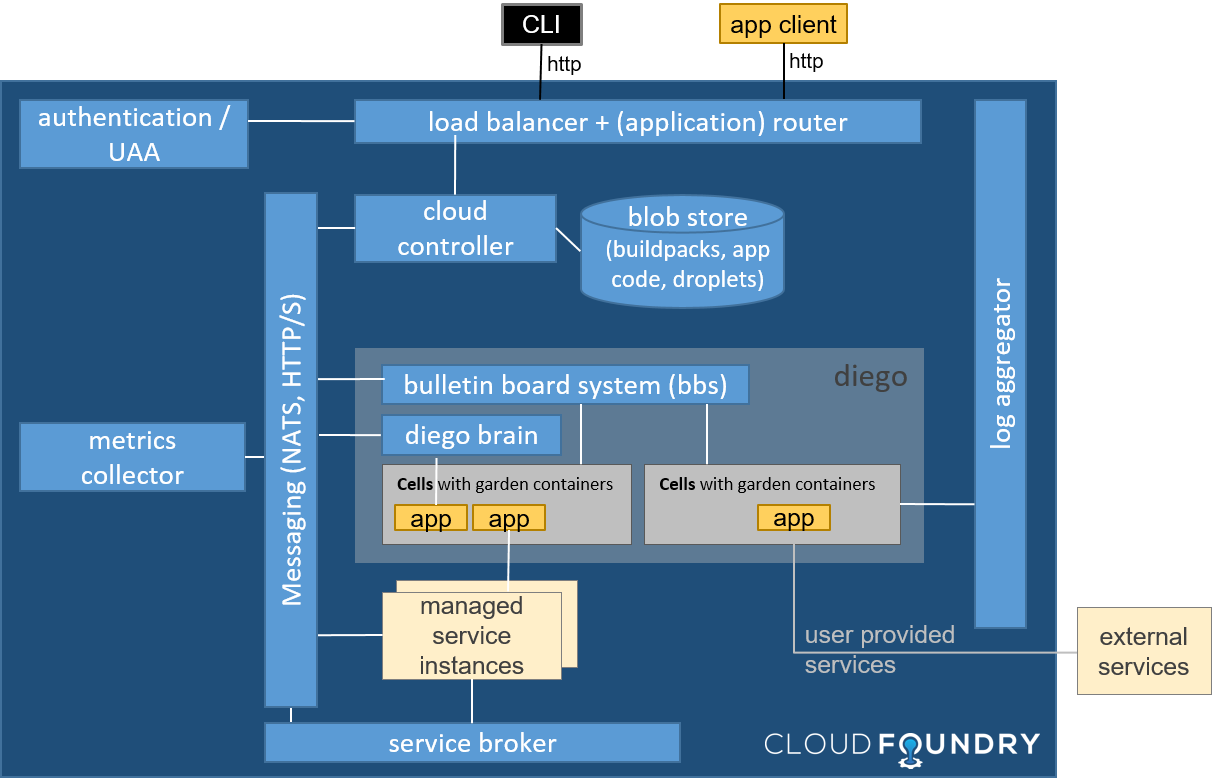
\includegraphics[width=0.8\textwidth]{../CloudFoundryBasics//images/CF_HL_Architecture}
  \end{figure}
\vspace{-5mm}
\vfill
\tiny
\colorlink{https://docs.cloudfoundry.org/concepts/architecture}{CF Components}
\\\colorlink{https://docs.cloudfoundry.org/concepts/diego/diego-architecture.html}{CF Diego Architecture}

\end{frame}


\begin{frame}{Deploy a Service to Cloud Foundry}
\begin{center}
\Huge DEMO
\end{center}
\end{frame}


\begin{frame}{Reference: CF commands to deploy a service}
	\begin{table}
	\scriptsize
	\begin{tabular}{|p{0.35\textwidth}|p{0.55\textwidth}|}
	\hline
	\codealt{cf api} \linebreak{} {\tiny \codealt{ https://api.cf.sap.hana.ondemand.com}}  &
	  Connect to a cloud foundry provider (URL of cloud controller).  \\ \hline
	\codealt{cf login [-u username -o org]}  &
	  Log in as user (use SAP domain user and password) and pass org \\ \hline
	\codealt{cf target [ -s space ]}  &
	  Show or set a target space (where cf apps are deployed)    \\ \hline
	\codealt{cf buildpacks} & Shows supported buildpack versions \\ \hline
	\codealt{cf apps} & Show running microservices \\ \hline
	\codealt{cf push [-n hostname]} & Push app in current directory to CF using local manifest \\ \hline
	\codealt{cf scale appname -i 2} & Scale app to 2 running instances \\ \hline
	\end{tabular}
	\end{table}

	\vfill
	Further References
	\begin{itemize}
	\item \colorlink{https://github.wdf.sap.corp/cc-devops-course/coursematerial/blob/master/Cheat_Sheets/CS_Merged.pdf}{Cloud Foundry CLI Cheat Sheet}
	\item \colorlink{https://plugins.cloudfoundry.org/}{Cloud Foundry CLI Plugins}
	\end{itemize}
\end{frame}


\begin{frame}[fragile]{Manifest.yml: deployment descriptor}
A manifest specifies application parameters to Cloud Foundry.\\
\vfill
\begin{block}{Example manifest.yml}
\begin{lstlisting}[language=yaml]
---
applications:
- name: bulletinboard-ads
  memory: 1G
  instances: 1
  path: target/bulletinboard-ads.war
  buildpack: https://gh.com/cf/java-buildpack.git#v4.6
\end{lstlisting}
\end{block}

\end{frame}


\begin{frame}{Deploy your Application: \codealt{cf push}}
	\begin{figure}
  	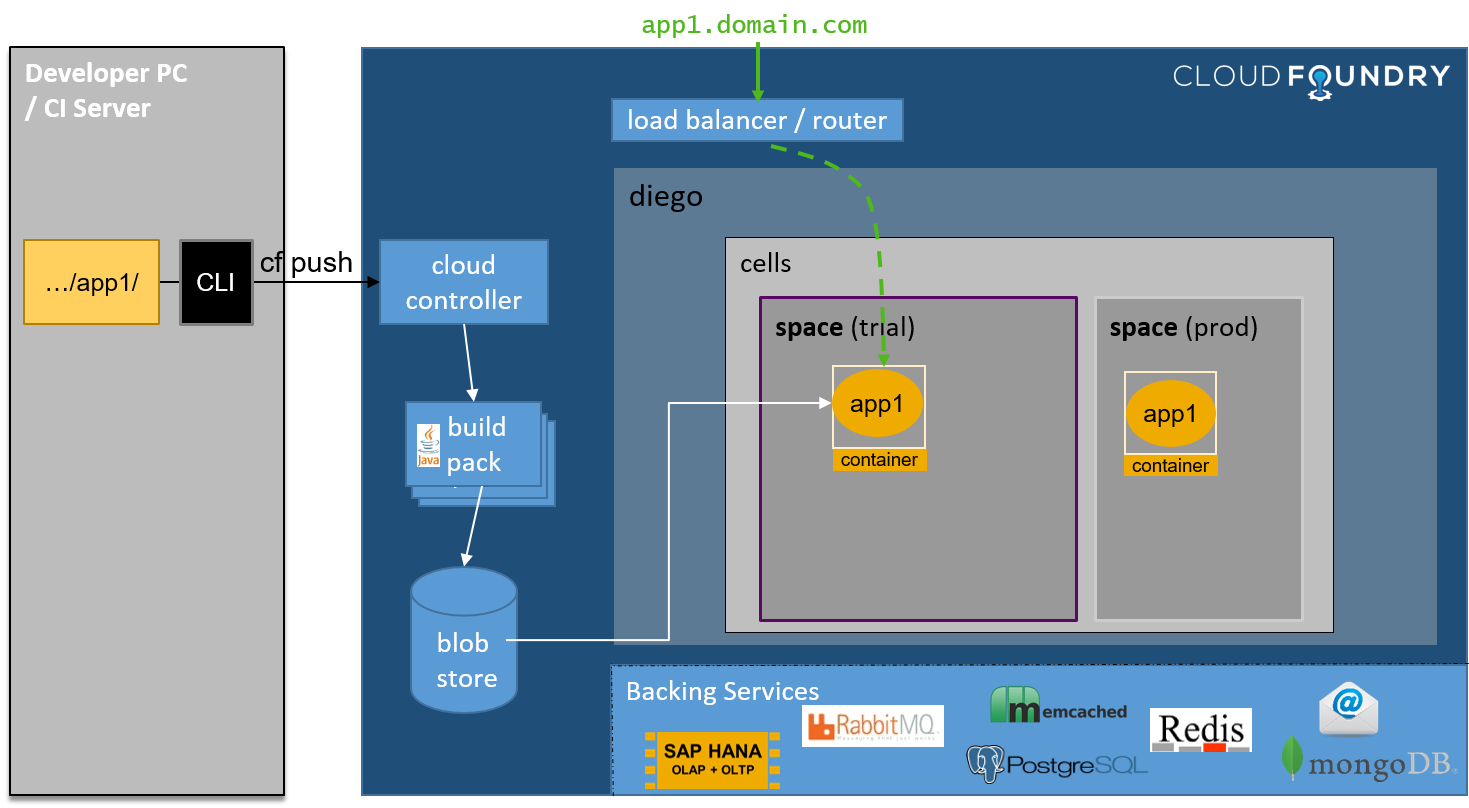
\includegraphics[width=0.9\textwidth]{../CloudFoundryBasics//images/CF_Basics_5_push_a}
	\end{figure}
\colorlink{https://docs.cloudfoundry.org/devguide/deploy-apps/start-restart-restage.html}{CF Doc - About Starting Applications}
\end{frame}

\begin{frame}{Scale your Application: \codealt{cf scale <appname>}}
	\begin{figure}
  	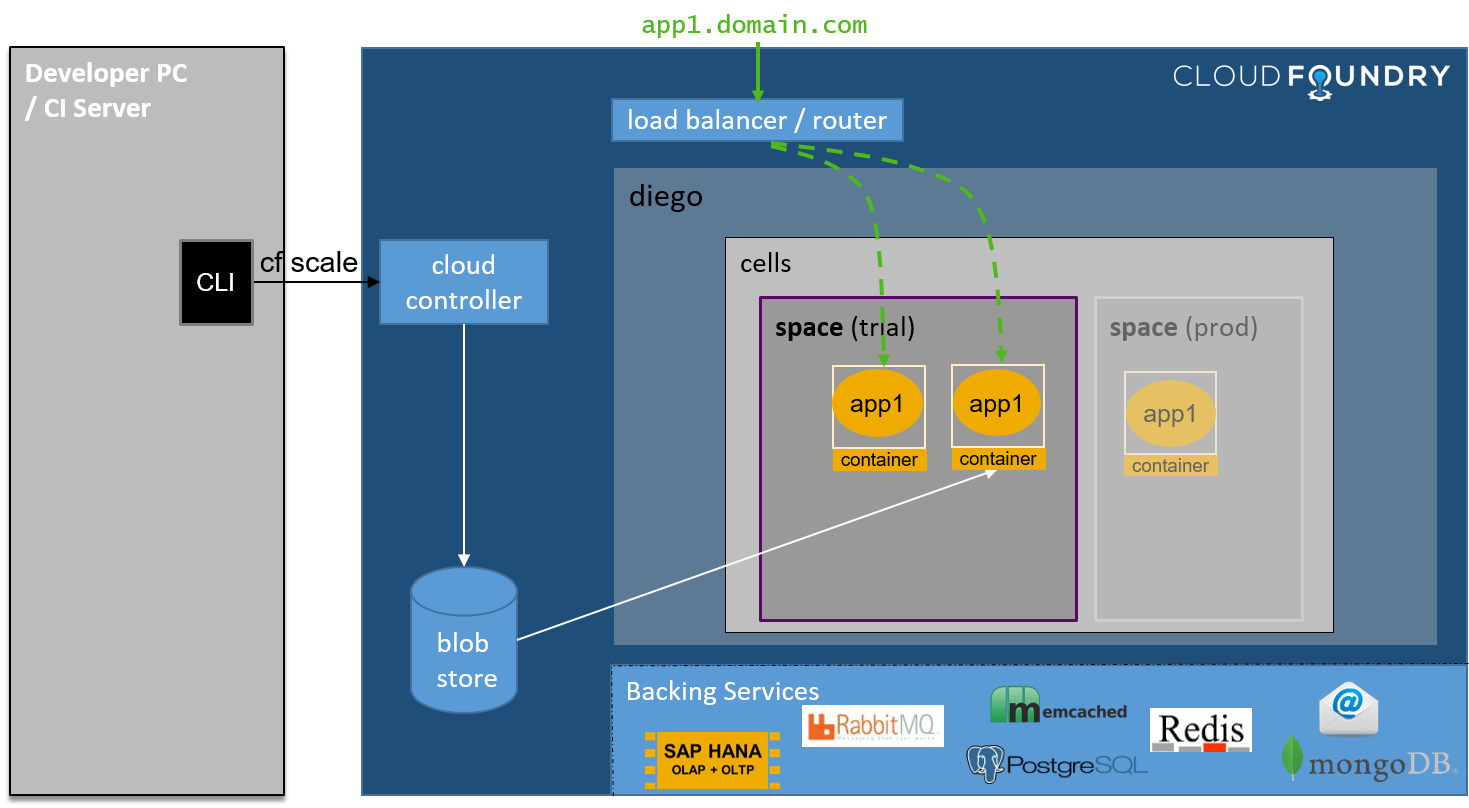
\includegraphics[width=0.9\textwidth]{../CloudFoundryBasics//images/CF_Basics_5b_scale_a}
	\end{figure}
\colorlink{https://docs.cloudfoundry.org/devguide/deploy-apps/cf-scale.html}{CF Doc - Scaling an Application}\\
\end{frame}


\begin{frame}{Orgs and Spaces}
\begin{columns}
\begin{column}{.50\textwidth}
\textbf{Org} defines resource quota, billing account, users etc. \\
\ \\
\textbf{Spaces}
	\small
	\begin{itemize}
		\item Spaces contain running apps
		\item Users are assigned to spaces, can deploy, start, stop, scale, ...
		\item Use \textbf{\codealt{cf push -n <hostname>}} \\ to specify unique route for your app \\ and to avoid URL conflicts 
	\end{itemize}
\end{column}
\begin{column}{.48\textwidth}
  	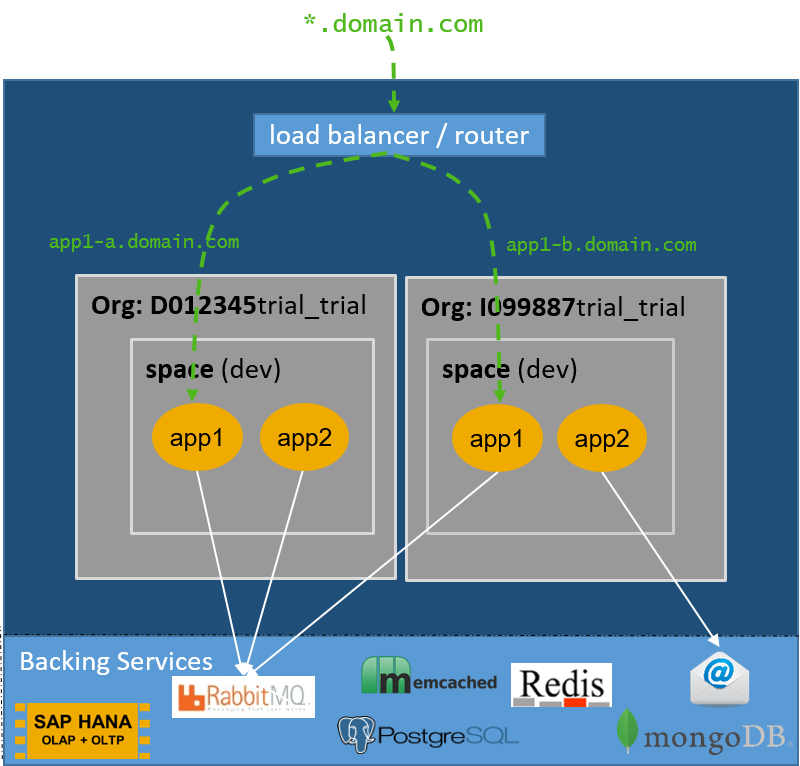
\includegraphics[width=1.0\textwidth]{../CloudFoundryBasics/images/CF_Basics_6_push-n_a}
	\scriptsize
	\vfill
	\colorlink{https://account.int.sap.hana.ondemand.com/cockpit\#/home/overview}{SAP CP Cockpit}
\end{column}
\end{columns}
\end{frame}

\begin{frame}{Exercise 6}
	\begin{figure}
		\includeGraphicsExerciseSix{width=0.8\textwidth}
	\end{figure}
	\colorlink{https://github.com/ccjavadev/cc-coursematerial/blob/master/CloudFoundryBasics/Exercise_6_DeployAdsOnCloudFoundry.md}{Exercise 6: Deploy Service to Cloud Foundry}
\end{frame}

\begin{frame}{References}
	\begin{itemize}
		\item \colorlink{https://docs.cloudfoundry.org/}{Cloud Foundry documentation}
		\item \colorlink{https://jam4.sapjam.com/groups/about_page/ApFhQ0NCGAzAtXQWsdqB3B}{Cloud Foundry JAM}
		\item \colorlink{https://help.sap.com/viewer/65de2977205c403bbc107264b8eccf4b/Cloud/en-US/9c7092c7b7ae4d49bc8ae35fdd0e0b18.html}{List of CF open source features supported on SAP Cloud Platform}
		\item \colorlink{https://account.int.sap.hana.ondemand.com/cockpit\#/home/overview}{SAP CP Cockpit - SAP internal}
		\item \colorlink{https://account.hana.ondemand.com/cockpit}{SAP CP Cockpit - external}		
		\item \colorlink{https://help.sap.com/viewer/65de2977205c403bbc107264b8eccf4b/Cloud/en-US/350356d1dc314d3199dca15bd2ab9b0e.html}{SAP CP - help portal}
		\item \colorlink{https://github.infra.hana.ondemand.com/cloudfoundry/cf-docs/wiki/CF-EU10-CANARY}{SAP CP Release Notes / Internal Documentation}
		\item \colorlink{https://wiki.wdf.sap.corp/wiki/display/CPC15N/SAP+Cloud+Platform+-+Internal+Pricelist+for+Neo+and+Cloud+Foundry+Services}{SAP CP - Internal Pricelist}
		\item \colorlink{https://jam4.sapjam.com/groups/ZBxGNs1cJ5Z7OVkQRwBM0G}{OneCP JAM - More SAP CP Presentations}
	\end{itemize}
\end{frame}




